\documentclass[12pt,a4paper,twoside]{article}
\usepackage[utf8]{inputenc}
\usepackage[spanish]{babel}
\usepackage{amsmath}
\usepackage{amsfonts}
\usepackage{amssymb}
\usepackage{graphicx}
\usepackage[left=2cm,right=2cm,top=2cm,bottom=2cm]{geometry}
\author{Yoleivys Delgado}
\title{\textbf{Movimiento de Proyectil con resistencia del aire}}

\begin{document}
\maketitle

En este movimiento, suponemos que un proyectil de masa m es lanzado a un tiempo $t=0$ desde la superficie de la tierra, formando un ángulo $\theta$ con la horizontal. Suponemos que  aparte de la fuerza de la gravedad, el proyectil esta sujeto a una fuerza de la resistencia del aire, la cual actúa opuesto a la dirección instantánea de movimiento y cuya magnitud es \textit{directamente proporcional} a su rapidez instantánea. Este modelo no es particularmente preciso para la fuerza de arrastre debido a la resistencia del aire, típicamente la magnitud de la fuerza de arrastre es directamente proporcional al cuadrado de la rapidez. Aunque este modelo permite obtener ecuaciones de movimientos tratables. Por lo que al usar este modelo podemos obtener una idea de como la resistencia del aire modifica las trayectorias del proyectil.\\ \\
Para el desarrollo de este tipo de movimiento se adoptara el sistemas de coordenadas cartesianas.\\ \\
La ecuación de movimiento del proyectil es escrito 

\begin{equation}
\centering
m\frac{d\textbf{v}}{dt} = mg -c\textbf{v}
\end{equation}

Donde la velocidad del proyectil es $\textbf{v}=(v_{x},v_{y})$ y la aceleración de la gravedad es $g=(0,-g)$, c es una constante positiva dada por $c=mg/v_{t}$, siendo $v_{t}$  la velocidad terminal del proyectil.\\
La velocidad terminal, es la velocidad mas alta que puede alcanzar un objeto cuando cae a través de un fluido.Se produce cuando la suma de la fuerza de arrastre ($F_{d}$) y la de flotabilidad ($F_{G}$) es igual a la fuerza de gravedad actuando en el objeto. Si no se considera los efectos de flotabilidad, la velocidad terminal esta dada por: 
\begin{equation}
\centering 
v_{t}= \sqrt{\frac{2mg}{\rho AC_{d}}}
\end{equation}

Donde 
\begin{itemize}
\item $v_{t}$ representa la velocidad terminal
\item $m$ es la masa del proyectil
\item $g$ es la aceleración debido a la gravedad
\item $C_{d}$ es el coeficiente de arrastre 
\item $\rho$  es la densidad del fluido en el cual el proyectil cae
\item A es el área proyectada del proyectil
\end{itemize}

En forma de componentes la ecuación $1$ se puede escribir como:
\begin{eqnarray}
\frac{dv_{x}}{dt} = -g\frac{v_{x}}{v_{t}} \\
\frac{dv_{y}}{dt} = -g (1+\frac{v_{y}}{v_{t}})
\end{eqnarray}

Las ecuaciones 3 y 4 pueden solucionarse utilizando métodos numéricos, como el método de integración de  Euler. Este es un método de  aproximación de primer orden para resolver ecuaciones diferenciales ordinarias (EDO) a partir de  valores inicial dados $ dy/dx = f(x,y)$ y  $(x_{0})= y_{0}$. El método parte de un desarrollo de Taylor de una función $f(x,y)$ alrededor de un punto y   conociendo los valores de la función y su derivada (las cuales deben ser continuas en este punto) se puede determinar el valor de la función en un punto inmediatamente siguiente usando la expresión: \\
\begin{eqnarray}
y_{n+1}= y_{n} + hf(x_{n},y_{n})
x_{n+1}= x_{n} + h
\end{eqnarray}

Donde h es lo que se le denomina paso del método y en primera instancia es considerado fijo.\\

Aplicando el método de Euler se obtiene  expresiones de la posición y velocidades horizontal y vertical del proyectil.Usando las ecuaciones 3 y 4. \\

\begin{eqnarray}
x(t_{n+1})= x(t_{n})+\Delta t v_{x}(t_{n})\\
v_{x}(t_{n+1}) = v_{x}(t_{n})[1-\frac{\Delta t}{m} c]
\end{eqnarray}
 
\begin{eqnarray}
y(t_{n+1})= y(t_{n})+\Delta t v_{y}(t_{n})\\
v_{y}(t_{n+1}) = v_{y}(t_{n})[1-\frac{\Delta t}{m} c] 
- \Delta t g
\end{eqnarray} \vspace{1cm}

\textbf{Ejemplo}\\
Obtener la trayectoria horizontal y vertical de un proyectil esférico de masa $m=0.5$ y radio $r=0.5$, que es lanzado desde la superficie de la tierra a un ángulo $\theta = 45^{\circ}$ y diferentes velocidades iniciales $v_{0} = (2,4,6,8,10)\hspace{0.2 cm} m/s$, y su movimiento se encuentra afectado por la resistencia del aire.\\
 
Para la solución numérica de este  problema se aplicaron las ecuaciones 6-9  y se obtuvieron las gráficas para las diferentes velocidades iniciales como se muestra en la figura (\ref{fig:figura1}).

\newpage
\begin{figure}[h]
\centering
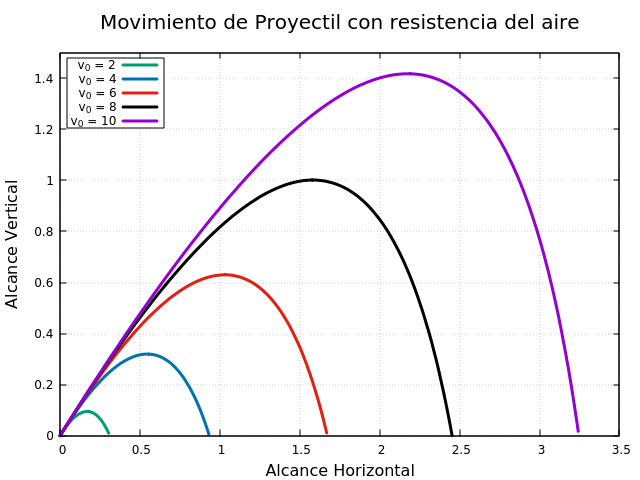
\includegraphics[width=10cm]{Imagen.png} 
\caption{Trayectorias seguida por un proyectil lanzados a diferentes velocidades y que se encuentra afectado por la resistencia del aire.}
\label{fig:figura1}
\end{figure}

los códigos de gnuplot y Fortran utilizados para la realización del ejercicio y graficación del mismo se presentan en la figura (\ref{fig:figura2}) y figura (\ref{fig:figura3})\\

\begin{figure}[h]
 \centering 
\begin{verbatim}
set title 'Movimiento de Proyectil con resistencia del aire'
set title font ",15" norotate
set xlabel "Alcance Horizontal"
set xlabel font "Verdana,12"
set ylabel "Alcance Vertical"
set ylabel font "Verdana,12"
set style data lines       # Todas las graficas las pone con lineas
set xrange [0:3.5]
set yrange [0:1.5]
set grid
set key left box
plot "friccion.dat" index 0 using 2:3 ls 2 lw 3 title "v_{0} = 2 ",\
"friccion.dat" index 1 using 2:3 ls 6 lw 3 title "v_{0} = 4",\
"friccion.dat" index 2 using 2:3 ls 7 lw 3 title "v_{0} = 6",\
"friccion.dat" index 3 using 2:3 ls 8 lw 3 title "v_{0} = 8",\
"friccion.dat" index 4 using 2:3 ls 9 lw 3 title " v_{0} = 10"
\end{verbatim}
\caption{Codigo gnuplot de la gráfica de la figura 1}
\label{fig:figura2}
\end{figure}

\newpage
 
\begin{verbatim}
program resistencia
  !Este programa estudia el movimiento de proyectil con resistencia del aire
  !donde la aceleración varia con la velocidad y se utiliza el metodo de euler
  !los dos primeros puntos del movimiento es tomado de acorde a un movimiento
  !sin friccion del aire.
  
  implicit none
  ! g, rho_a, m--------- gravedad, densidad del aire y masa del proyectil.
  ! cd, r -------------- coeficiente de arraste  y radio de la esfera.
  ! theta, dt----------- angulo de lanzamiento y intervalos de tiempos.

  !Definición de constantes 
  real, parameter:: g=9.8, pi=3.1415927, rho_a=1.128, cd =0.45, dt=0.01
  real, parameter:: m=0.5, theta = 45., r = 0.5
  integer, parameter:: size=1000
  integer::i,j

  !Definición de variables
  !vt, v0 -------- velocidad terminal e inicial del proyectil.
  !t,x,y,v_x,v_y---tiempo, posiciones y velocidades del proyectil.
  
  real::vt,a,C,v0
  real, dimension(0:size)::t, x, y, v_x, v_y
  

  !Calculo de la velocidad terminal
  
  vt= sqrt((2*m*g)/(rho_a*pi*r**2*cd))
  
  C = m*g / vt
   
  ! convirtiendo ángulo a radianes
     a = theta * pi / 180.0
  
   open(1, file='friccion.dat', status='unknown')  

   !loop para trabajar con diferentes velocidades 

do j=2,10,2
    
     v0=real(j)
     ! Primeros dos puntos del movimiento suponiendo que no hay fricción  
     t(0)=0.
     
     x(0)=0.
     y(0)=0.
     
     v_x(0)=v0*cos(a)
     v_y(0)=v0*sin(a)   
\end{verbatim}
 
\begin{figure}[h]
\centering
\begin{verbatim}
     write(1,1000) t(0), x(0), y(0), v_x(0), v_y(0)
     
     t(1)= t(0)+dt

     x(1) = x(0) + v0*t(1)*cos(a)
     y(1) = y(0) + v0*t(1)*sin(a)-0.5*g*t(1)**2
       
     v_x(1) = v0*cos(a)
     v_y(1) = v0*sin(a)-g*t(1)
     
    write(1,1000) t(1), x(1), y(1),v_x(1),v_y(1)

    ! loop para el movimiento con fricción  
    do i=2,size

     t(i) = t(i-1) + dt
         
     x(i) = x(i-1) + dt*v_x(i-1)
     y(i) = y(i-1) + dt*v_y(i-1)
     
     v_x(i)= v_x(i-1)*(1-(dt*C)/m)
     v_y(i)= v_y(i-1)*(1-(dt*C)/m)-dt*g
    
     if (y(i)<0.) exit 
      
     write(1,1000) t(i), x(i), y(i),v_x(i),v_y(i)
     1000 format(f18.15,5x,f18.15, 5x, f18.15, 5x, f18.15,5x,f18.15) 
     end do
  
     write(1,1100)
     1100 format(/)

     !descargar las variables para inicial con el siguiente loop
     do i=2,size
     t(i)=0.
     x(i)=0.
     y(i)=0.
     v_x(i)=0.
     v_y(i)=0.
     end do

  end do 
     close(1)
  

end program resistencia
\end{verbatim}
\caption{Codigo Fortran de las gráficas de la figura 1}
\label{fig:figura2}
\end{figure}
\end{document}